% exercise sheet with header on every page for math or close subjects
\documentclass[12pt]{article}
\usepackage[utf8]{inputenc} 
\usepackage{latexsym} 
\usepackage{multicol}
\usepackage{fancyhdr}
\usepackage{amsfonts} 
\usepackage{amsmath}
\usepackage{amssymb}
\usepackage{enumerate}
\usepackage{listings}
\usepackage{graphicx}
\usepackage{pdfpages}

% Shortcuts for bb, frak and cal letters
\newcommand{\E}{\mathbb{E}}
\newcommand{\V}{\mathbb{V}}
\renewcommand{\P}{\mathbb{P}}
\newcommand{\N}{\mathbb{N}}
\newcommand{\R}{\mathbb{R}}
\newcommand{\C}{\mathbb{C}}
\newcommand{\Z}{\mathbb{Z}}
\newcommand{\Pfrak}{\mathfrak{P}}
\newcommand{\Pfrac}{\mathfrak{P}}
\newcommand{\Bfrac}{\mathfrak{P}}
\newcommand{\Bfrak}{\mathfrak{B}}
\newcommand{\Fcal}{\mathcal{F}}
\newcommand{\Ycal}{\mathcal{Y}}
\newcommand{\Bcal}{\mathcal{B}}
\newcommand{\Acal}{\mathcal{A}}

% formating
\topmargin -1.5cm 
\textheight 24cm
\textwidth 16.0 cm 
\oddsidemargin -0.1cm

% Fancy Header on every Page
\pagestyle{fancy}
\lhead{\textbf{Programmierung for Engineers - Exercise 4}}
\rhead{Daniel Schäfer (2549458)\\ Dominik Weber (2548553)\\ Sina Vaghiri (2533563)}
\renewcommand{\headrulewidth}{1.2pt}
\setlength{\headheight}{60pt} 

\begin{document}
\pagenumbering{gobble}
\lstset{language=C}

\section{Aufgabe 1}
\subsection{Aufgabe131}
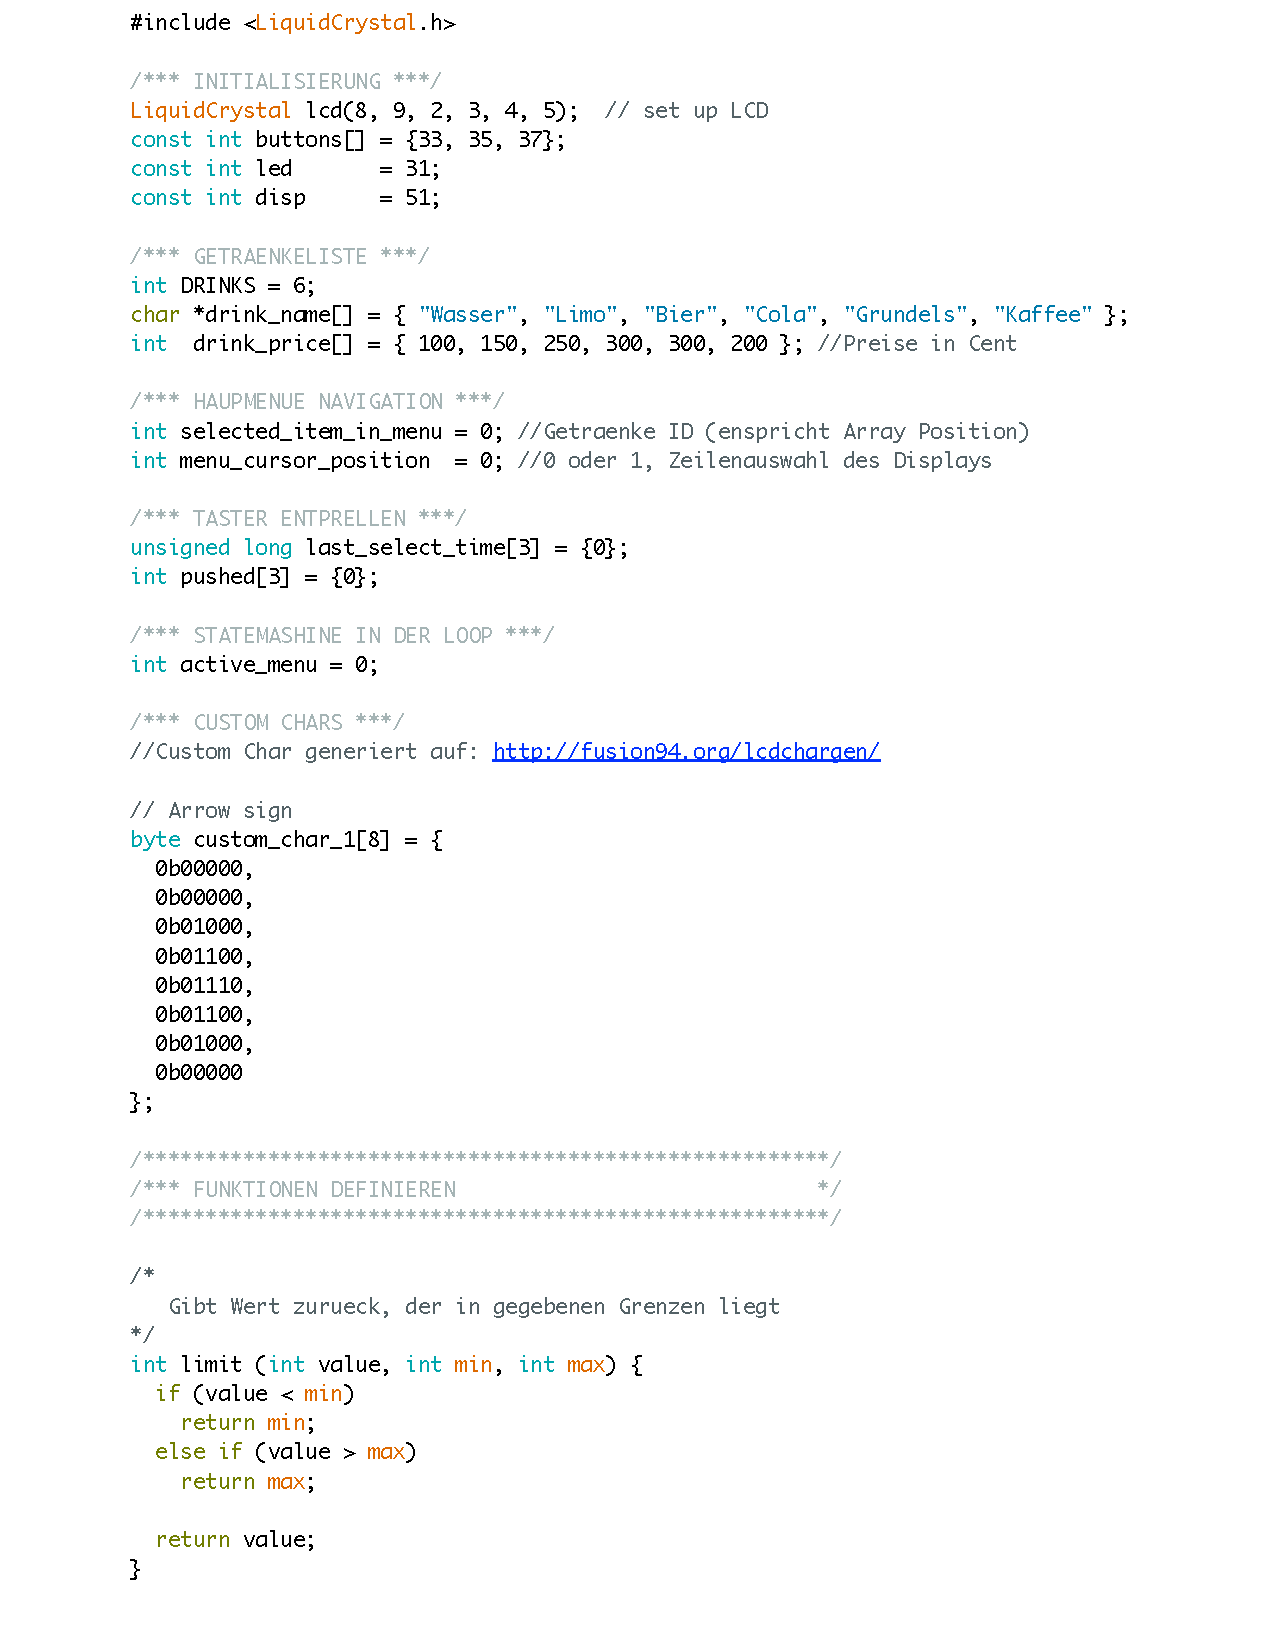
\includepdf[pages=-]{../drinkautomation131/drinkautomation131.pdf}

\subsection{Aufgabe132}
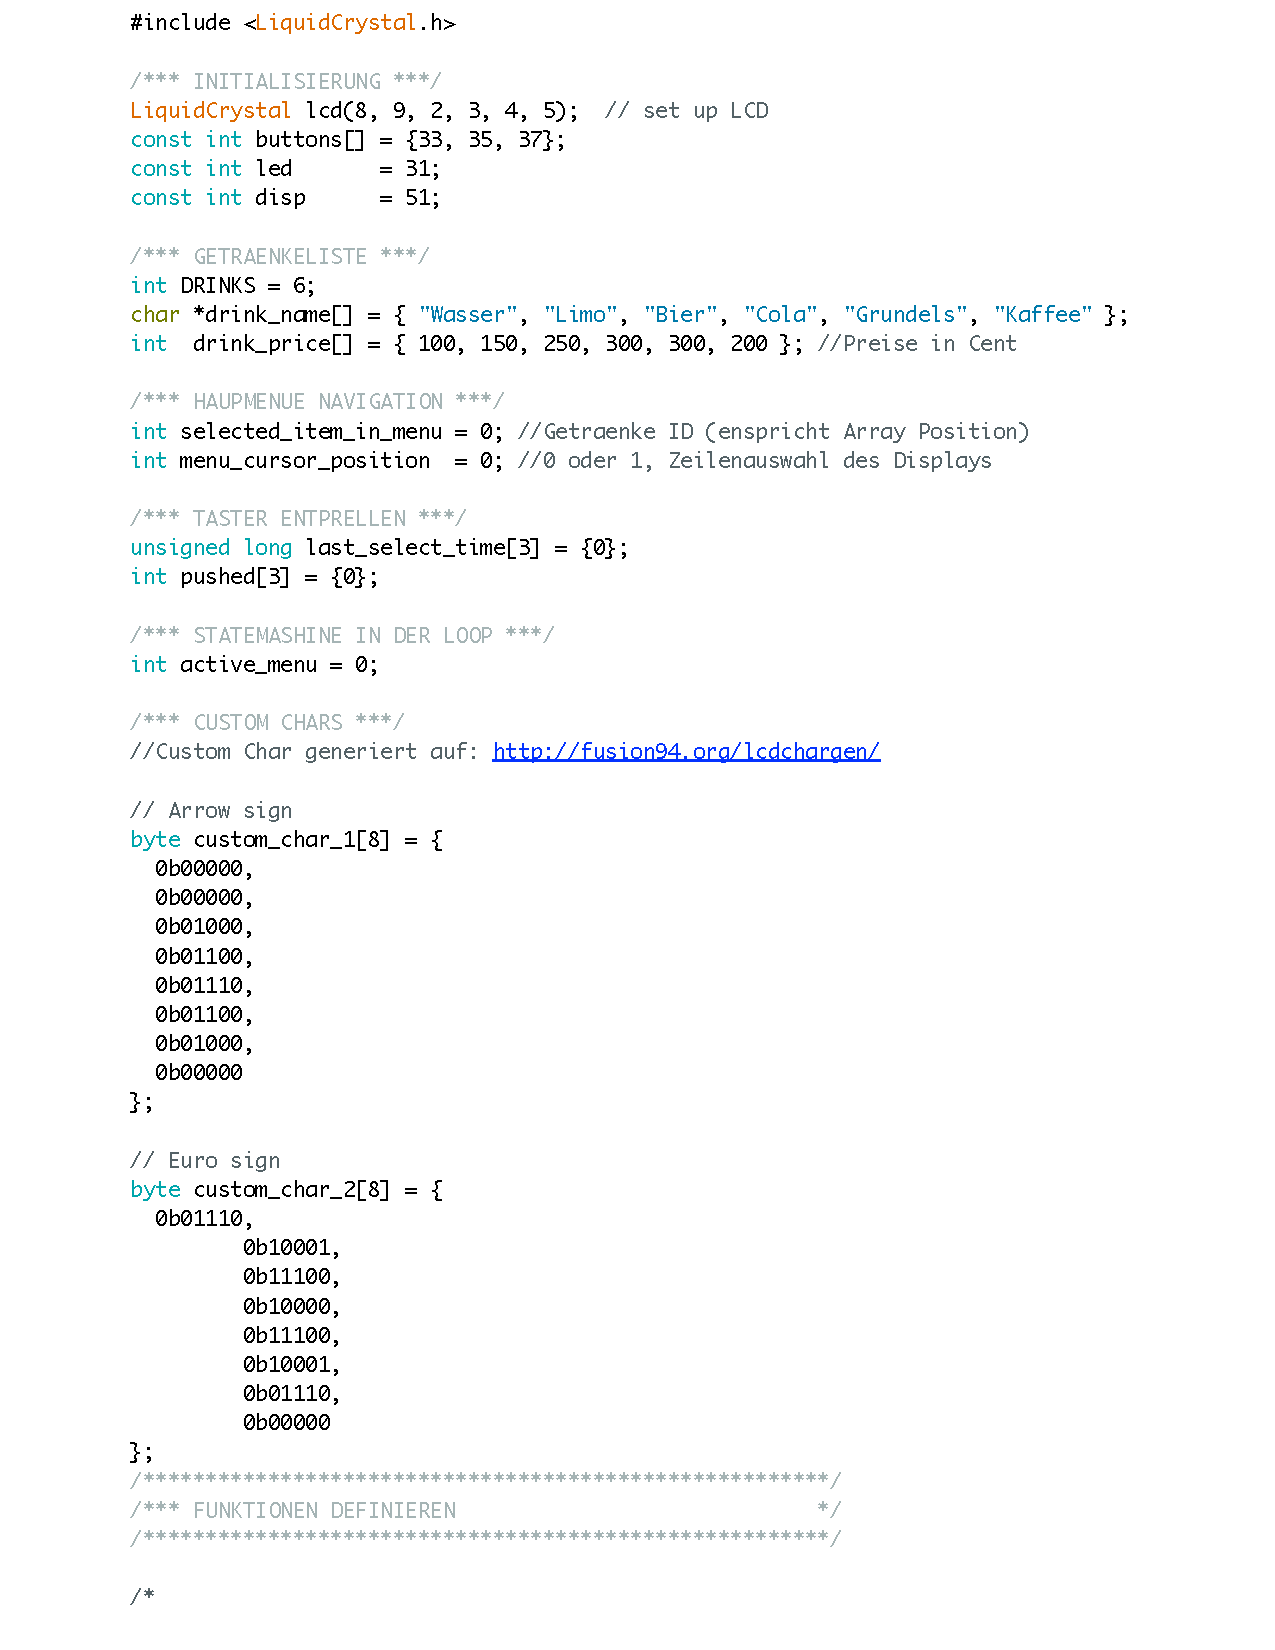
\includepdf[pages=-]{../drinkautomation132/drinkautomation132.pdf}

\subsection{Aufgabe133}
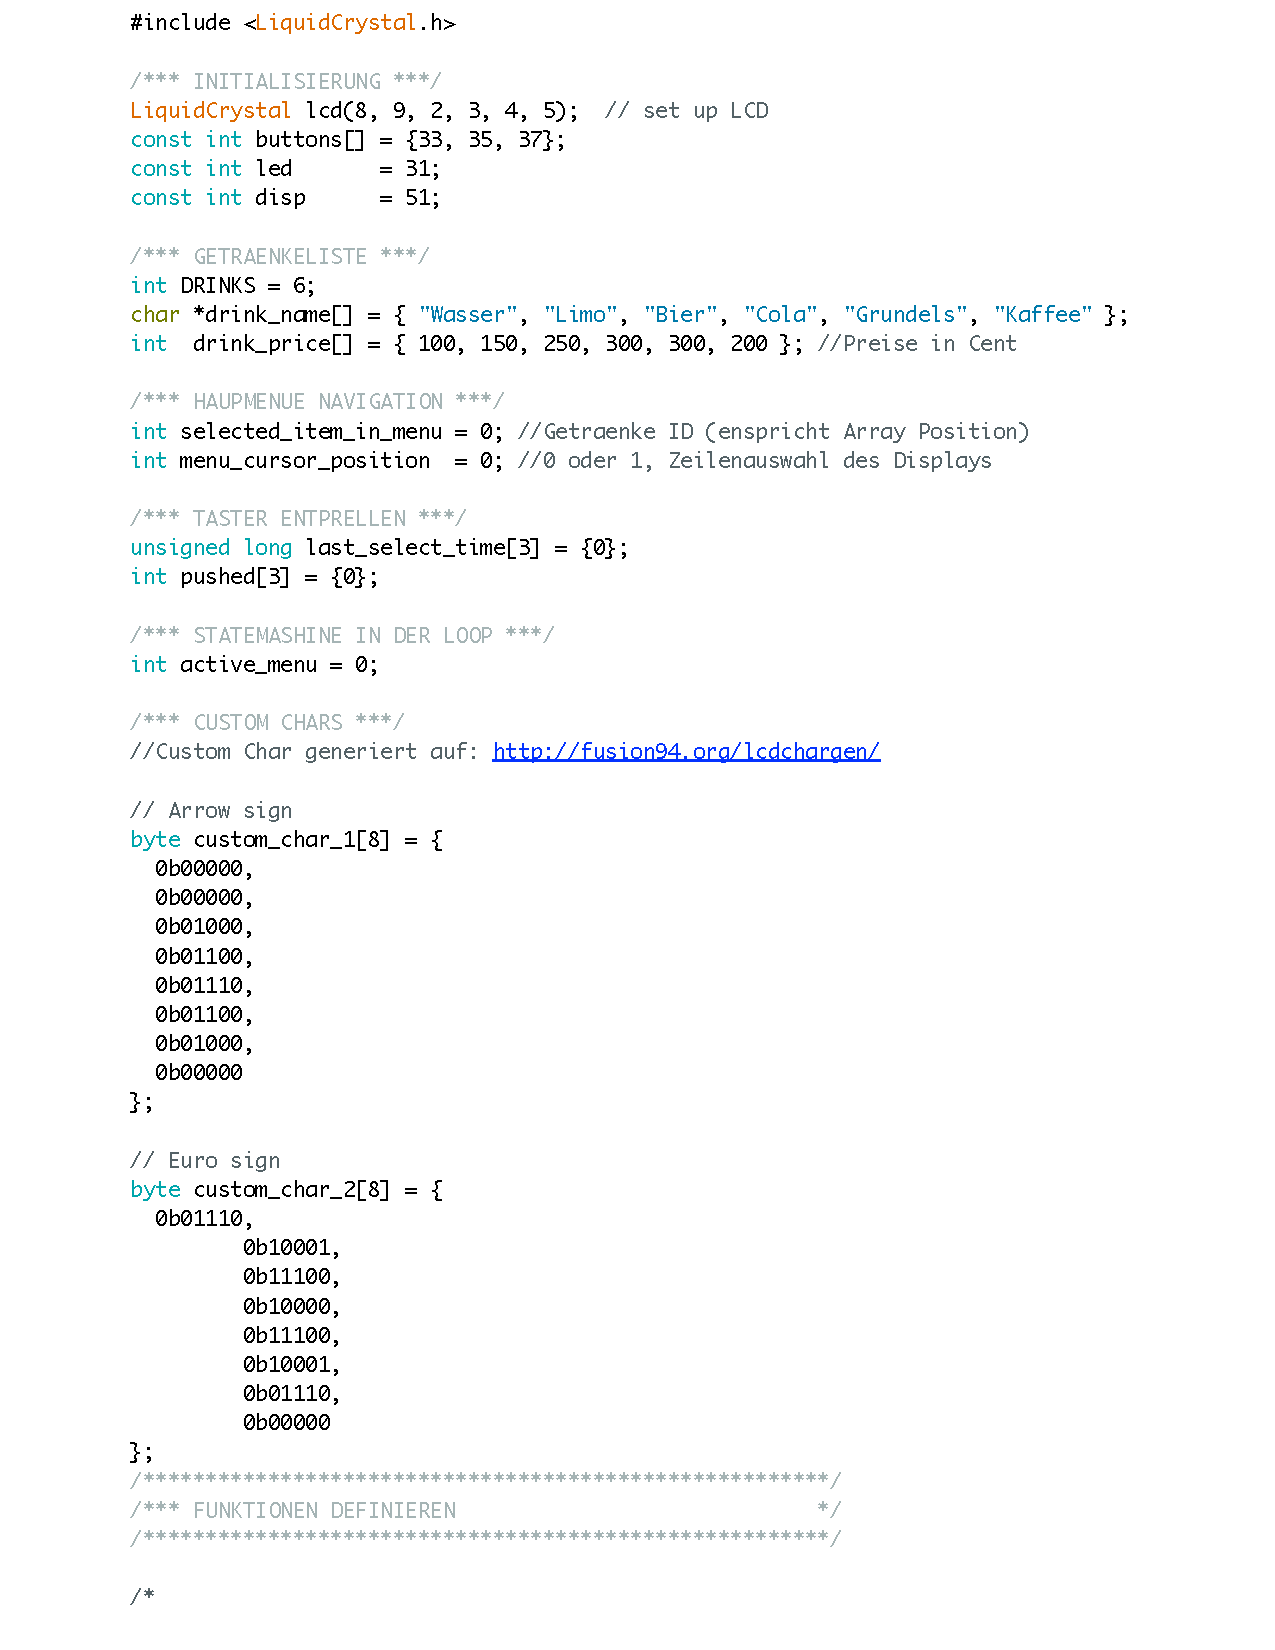
\includepdf[pages=-]{../drinkautomation133/drinkautomation133.pdf}

\subsection{Aufgabe14}
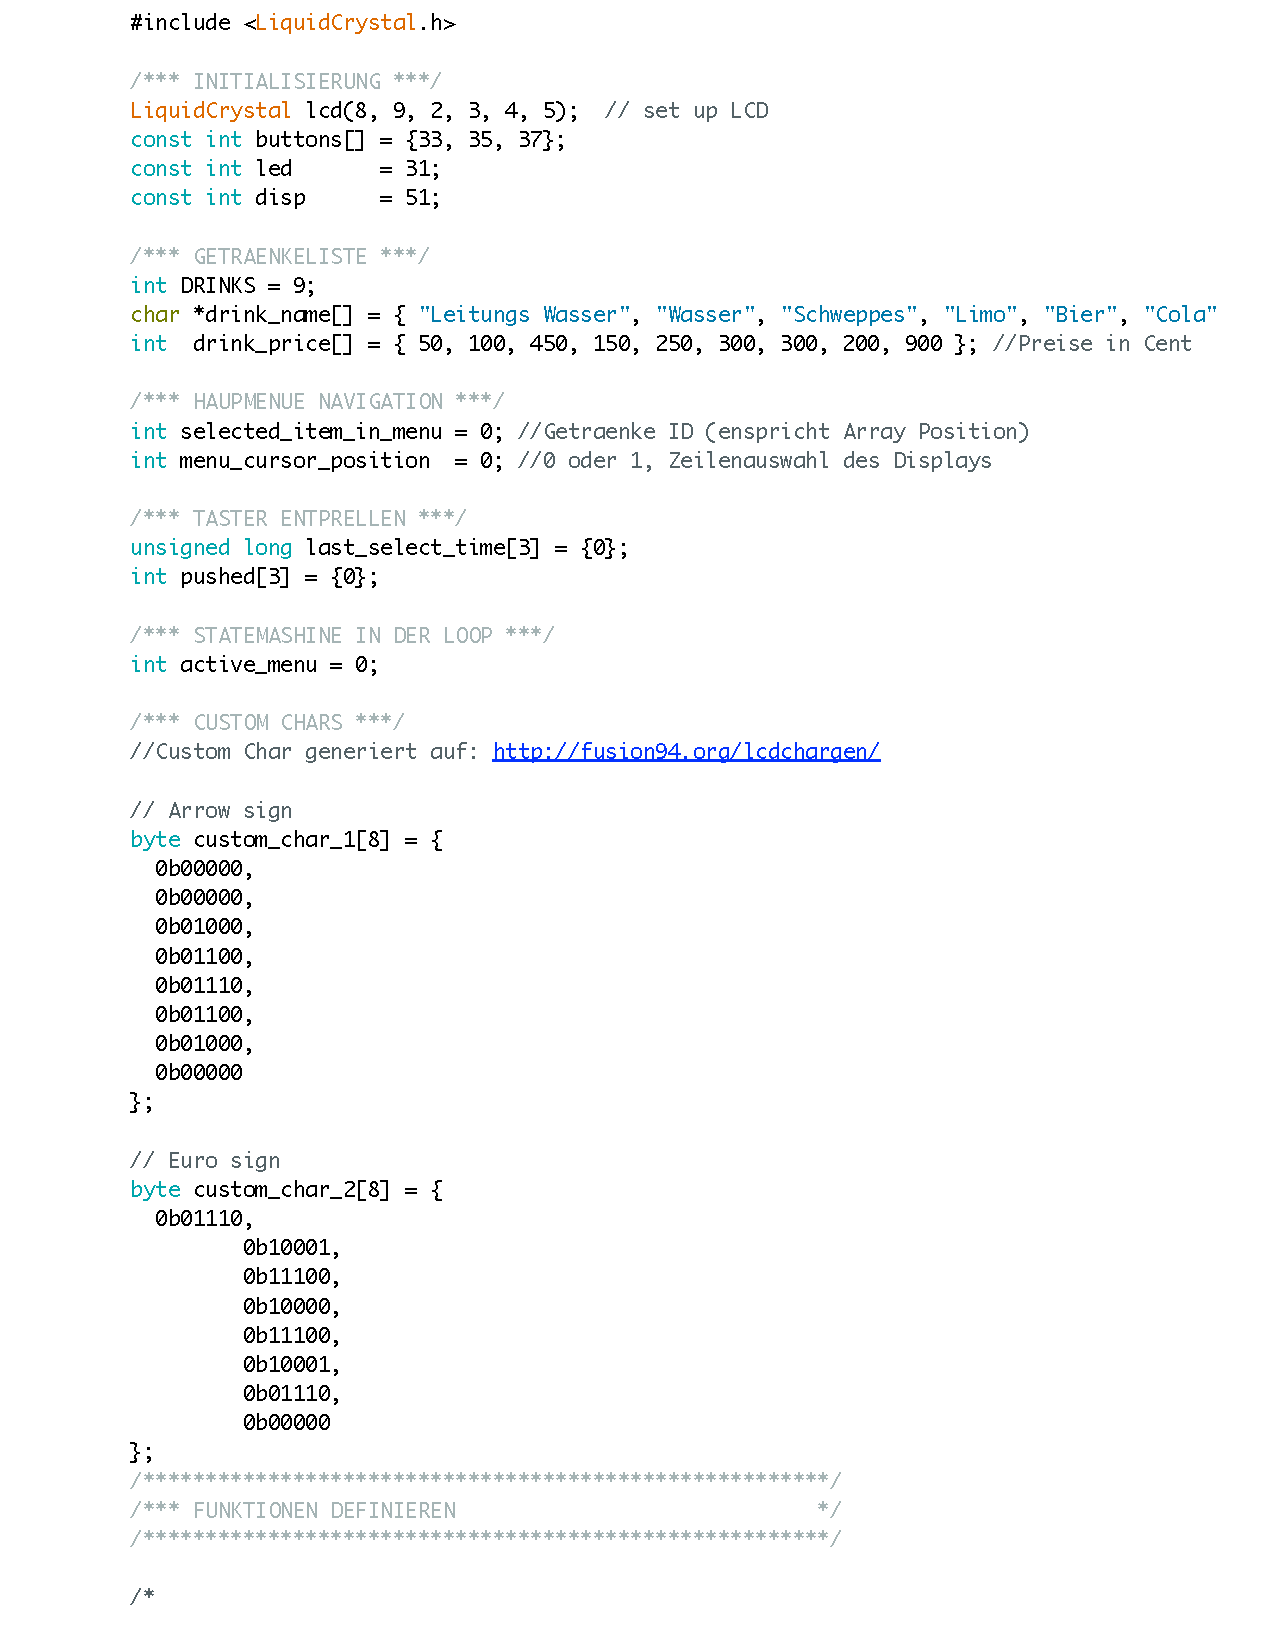
\includepdf[pages=-]{../drinkautomation14/drinkautomation14.pdf}

\subsection{Aufgabe15}
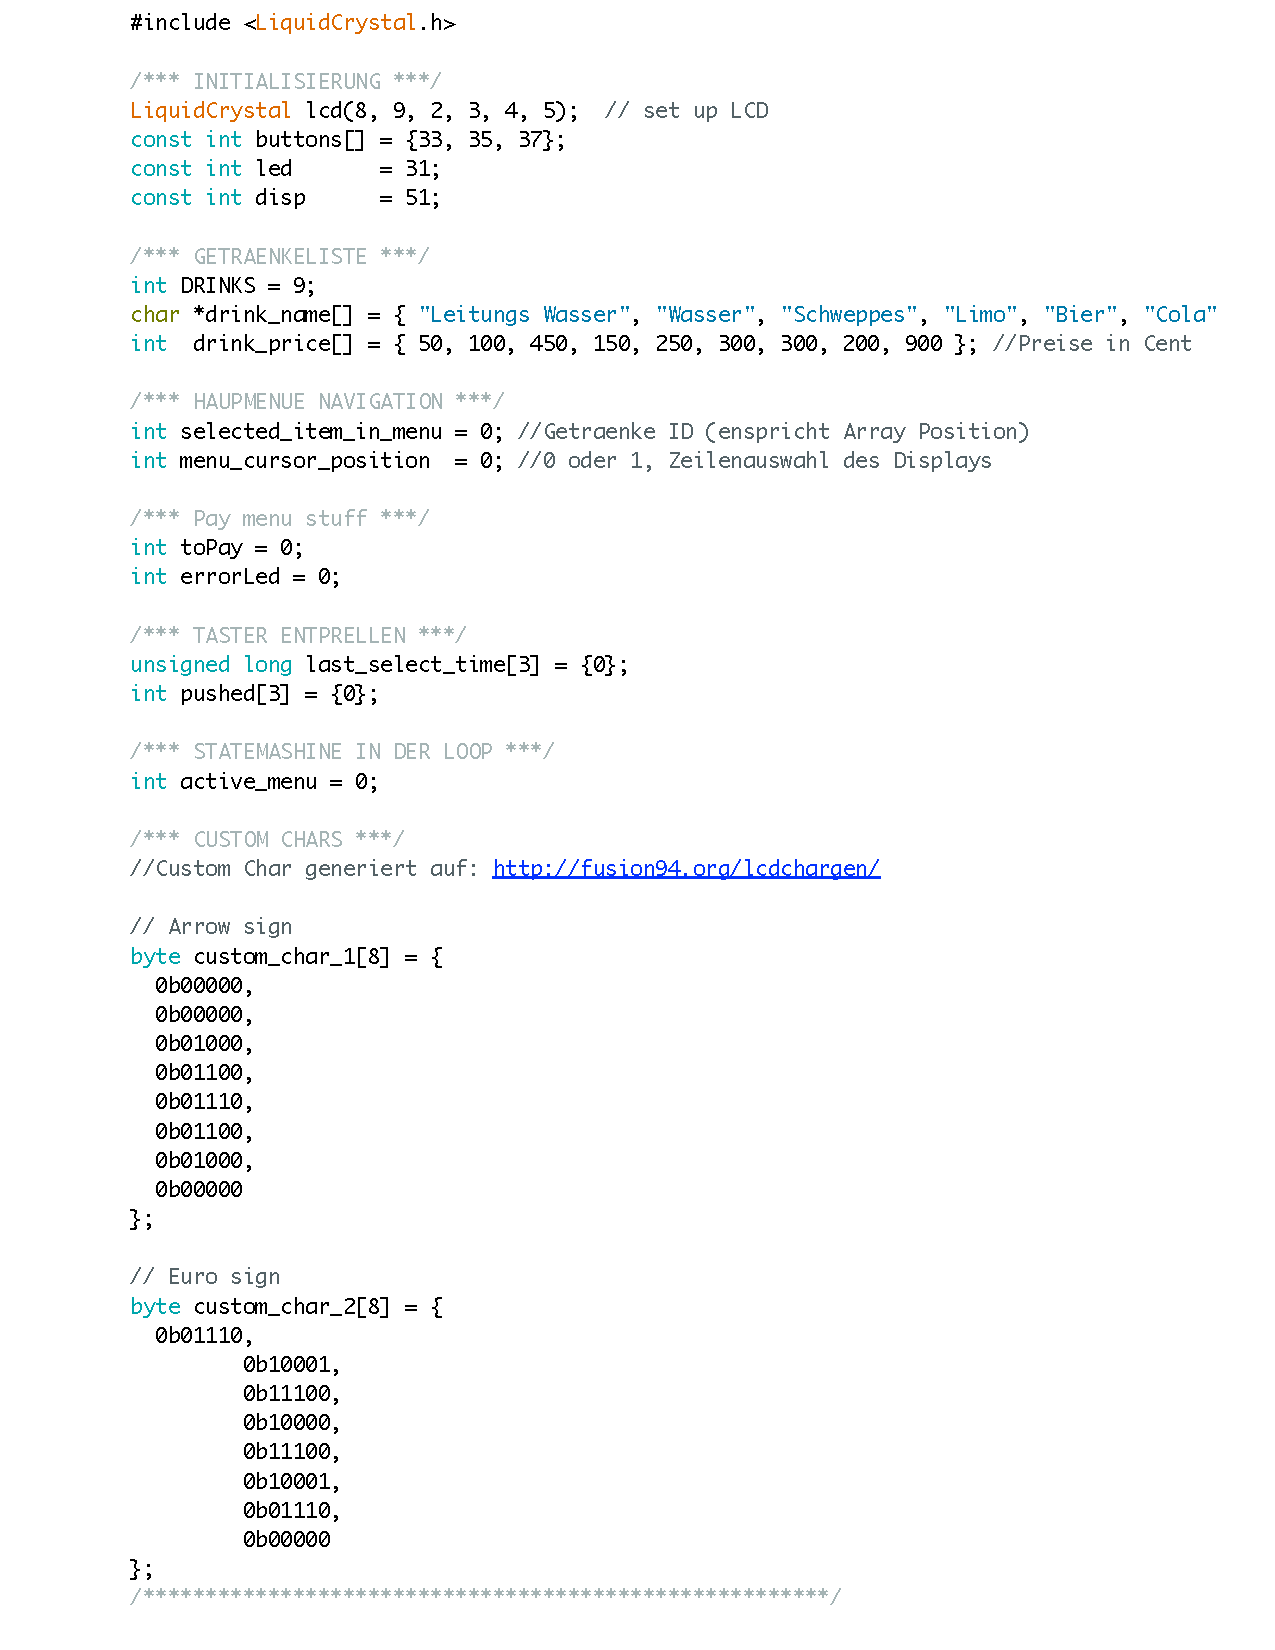
\includepdf[pages=-]{../drinkautomation15/drinkautomation15.pdf}

\subsection{Aufgabe16}
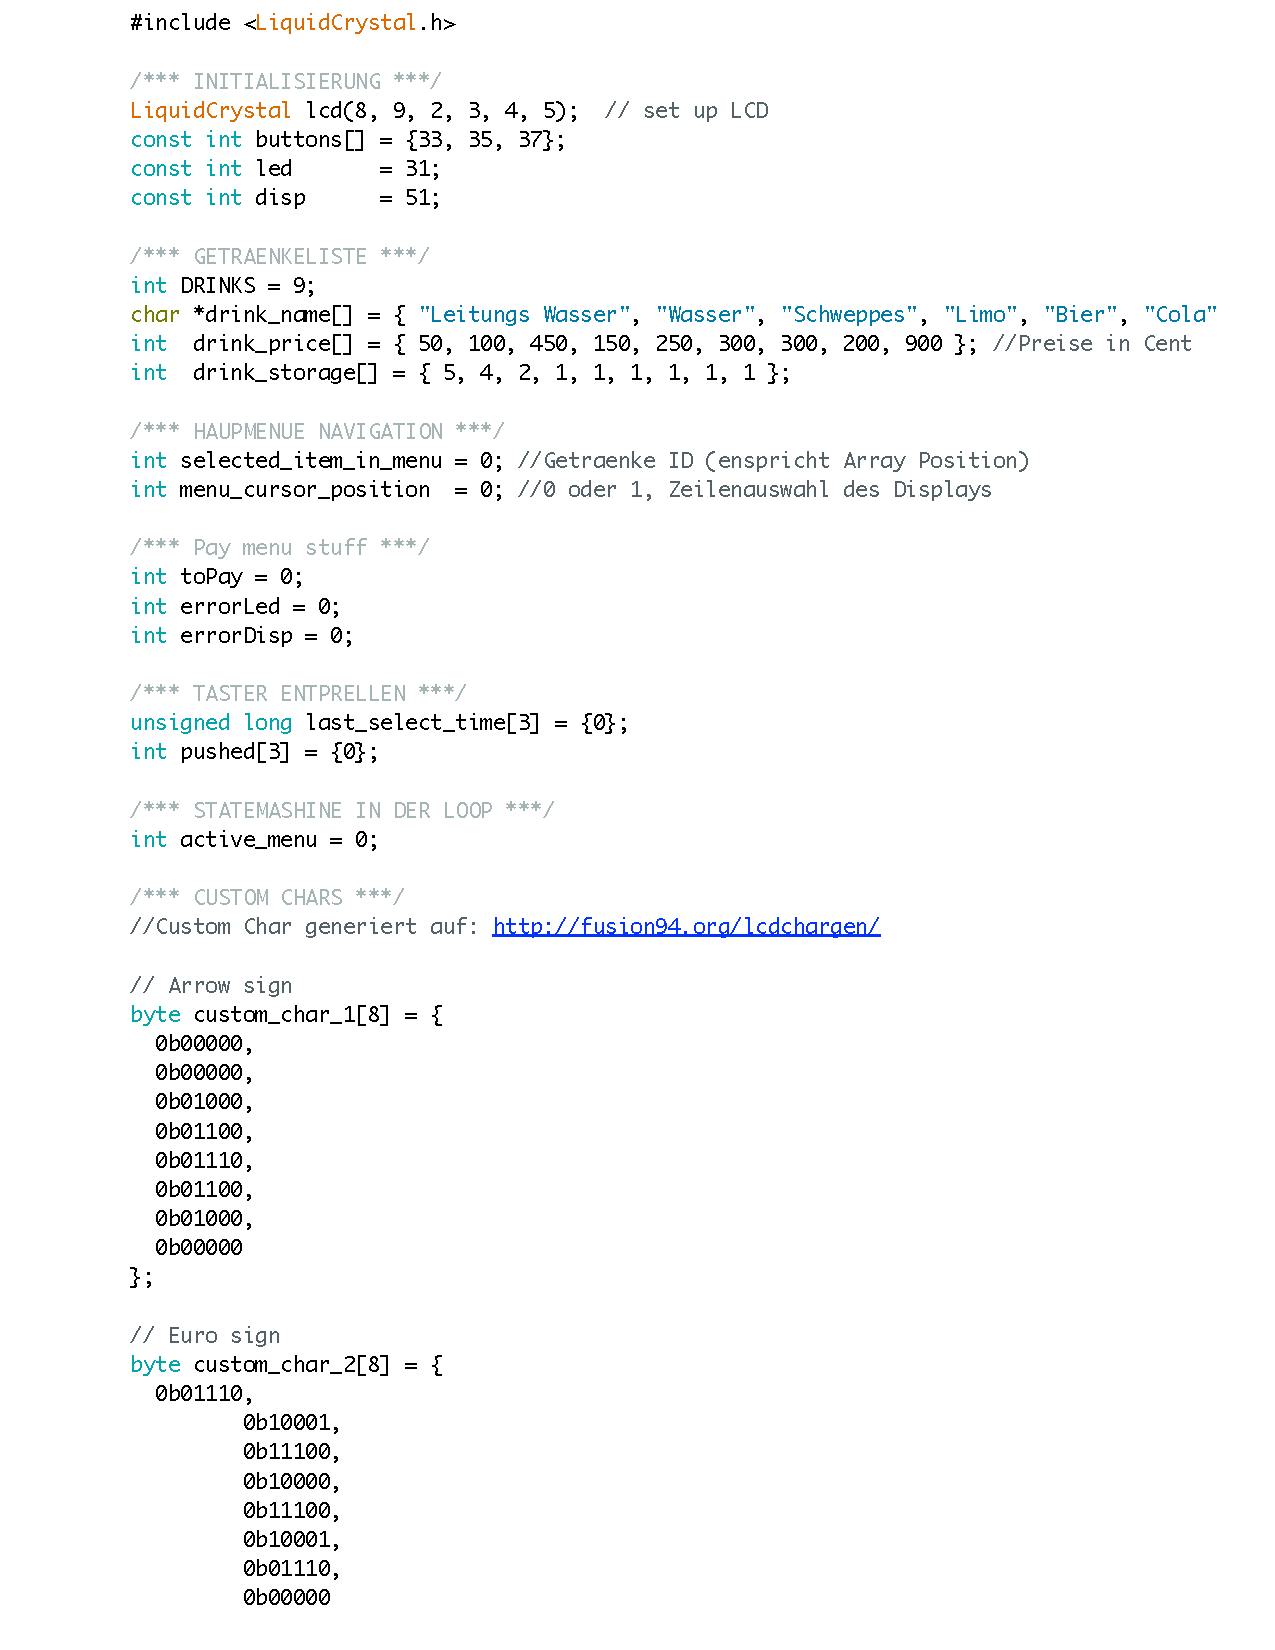
\includepdf[pages=-]{../drinkautomation16/drinkautomation16.pdf}

\subsection{Aufgabe17}
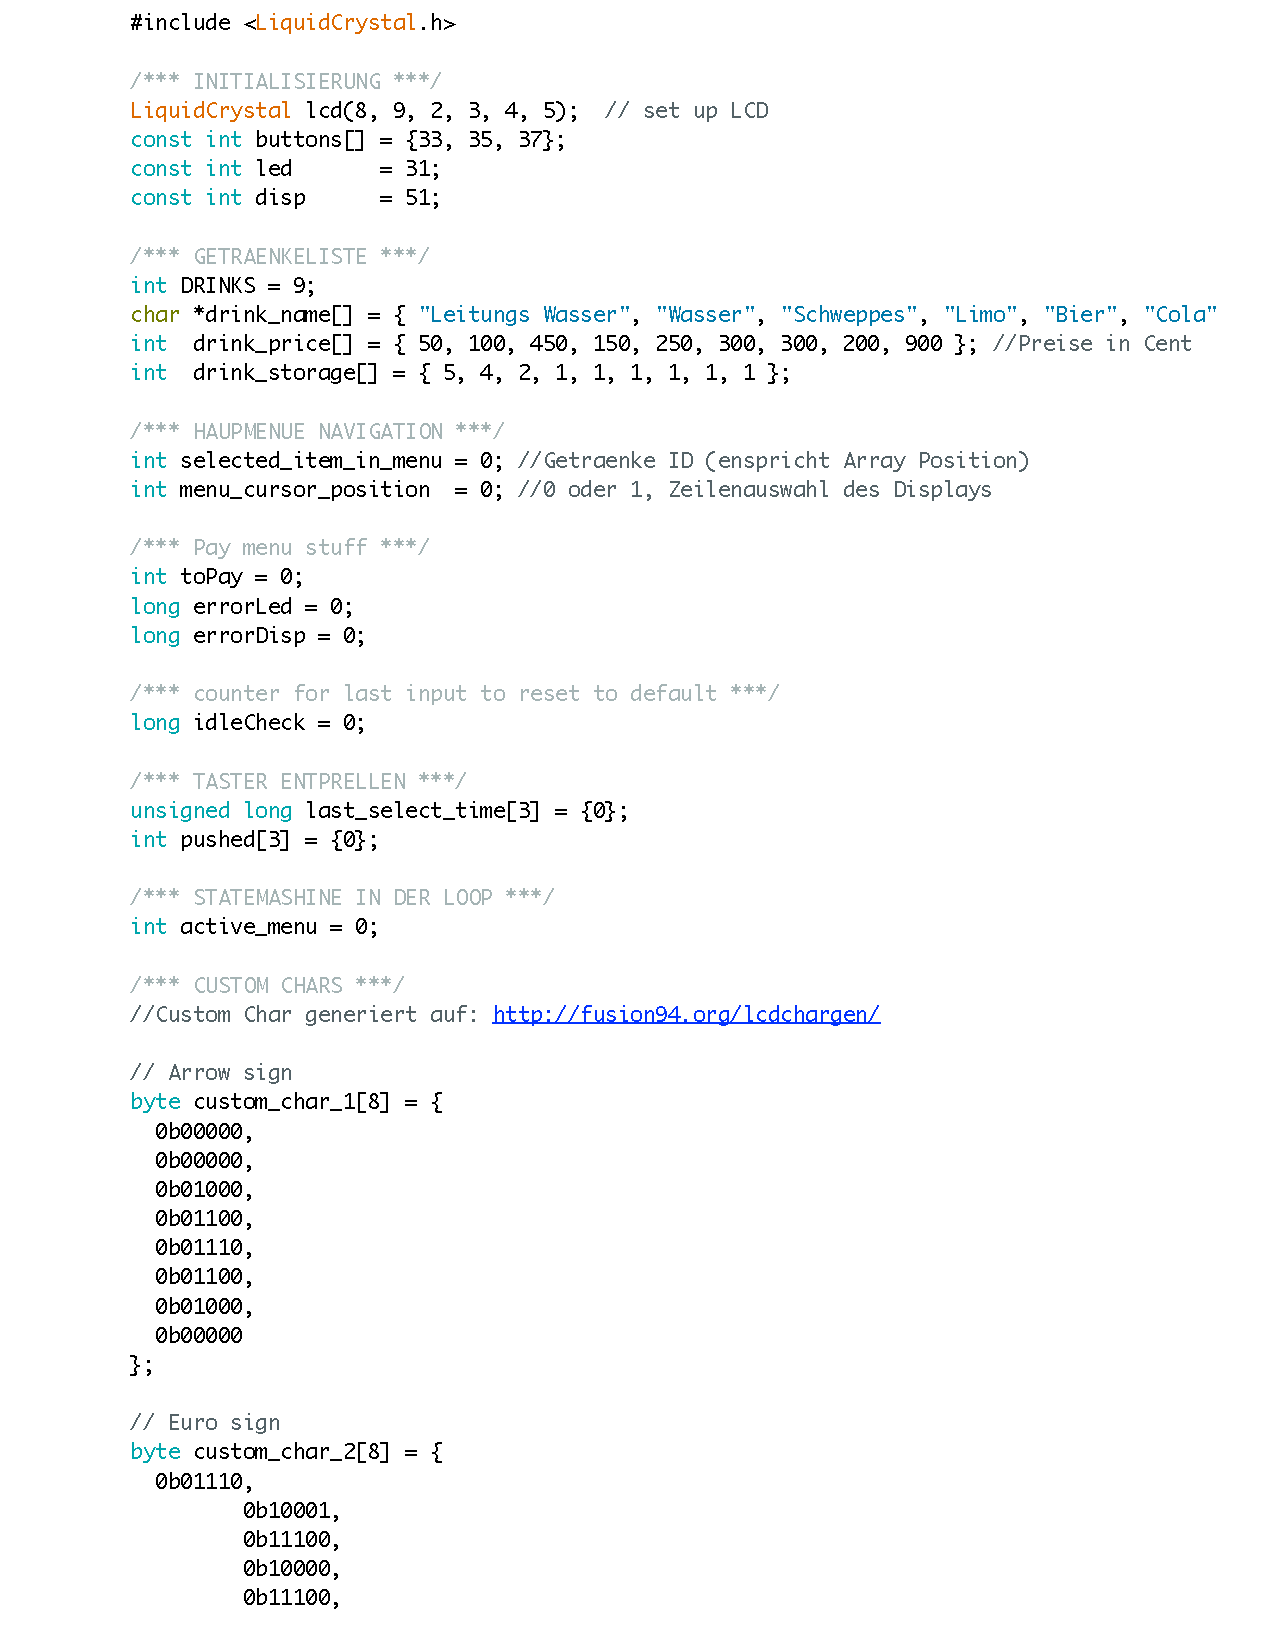
\includepdf[pages=-]{../drinkautomation17/drinkautomation17.pdf}

\section{Aufgabe2}
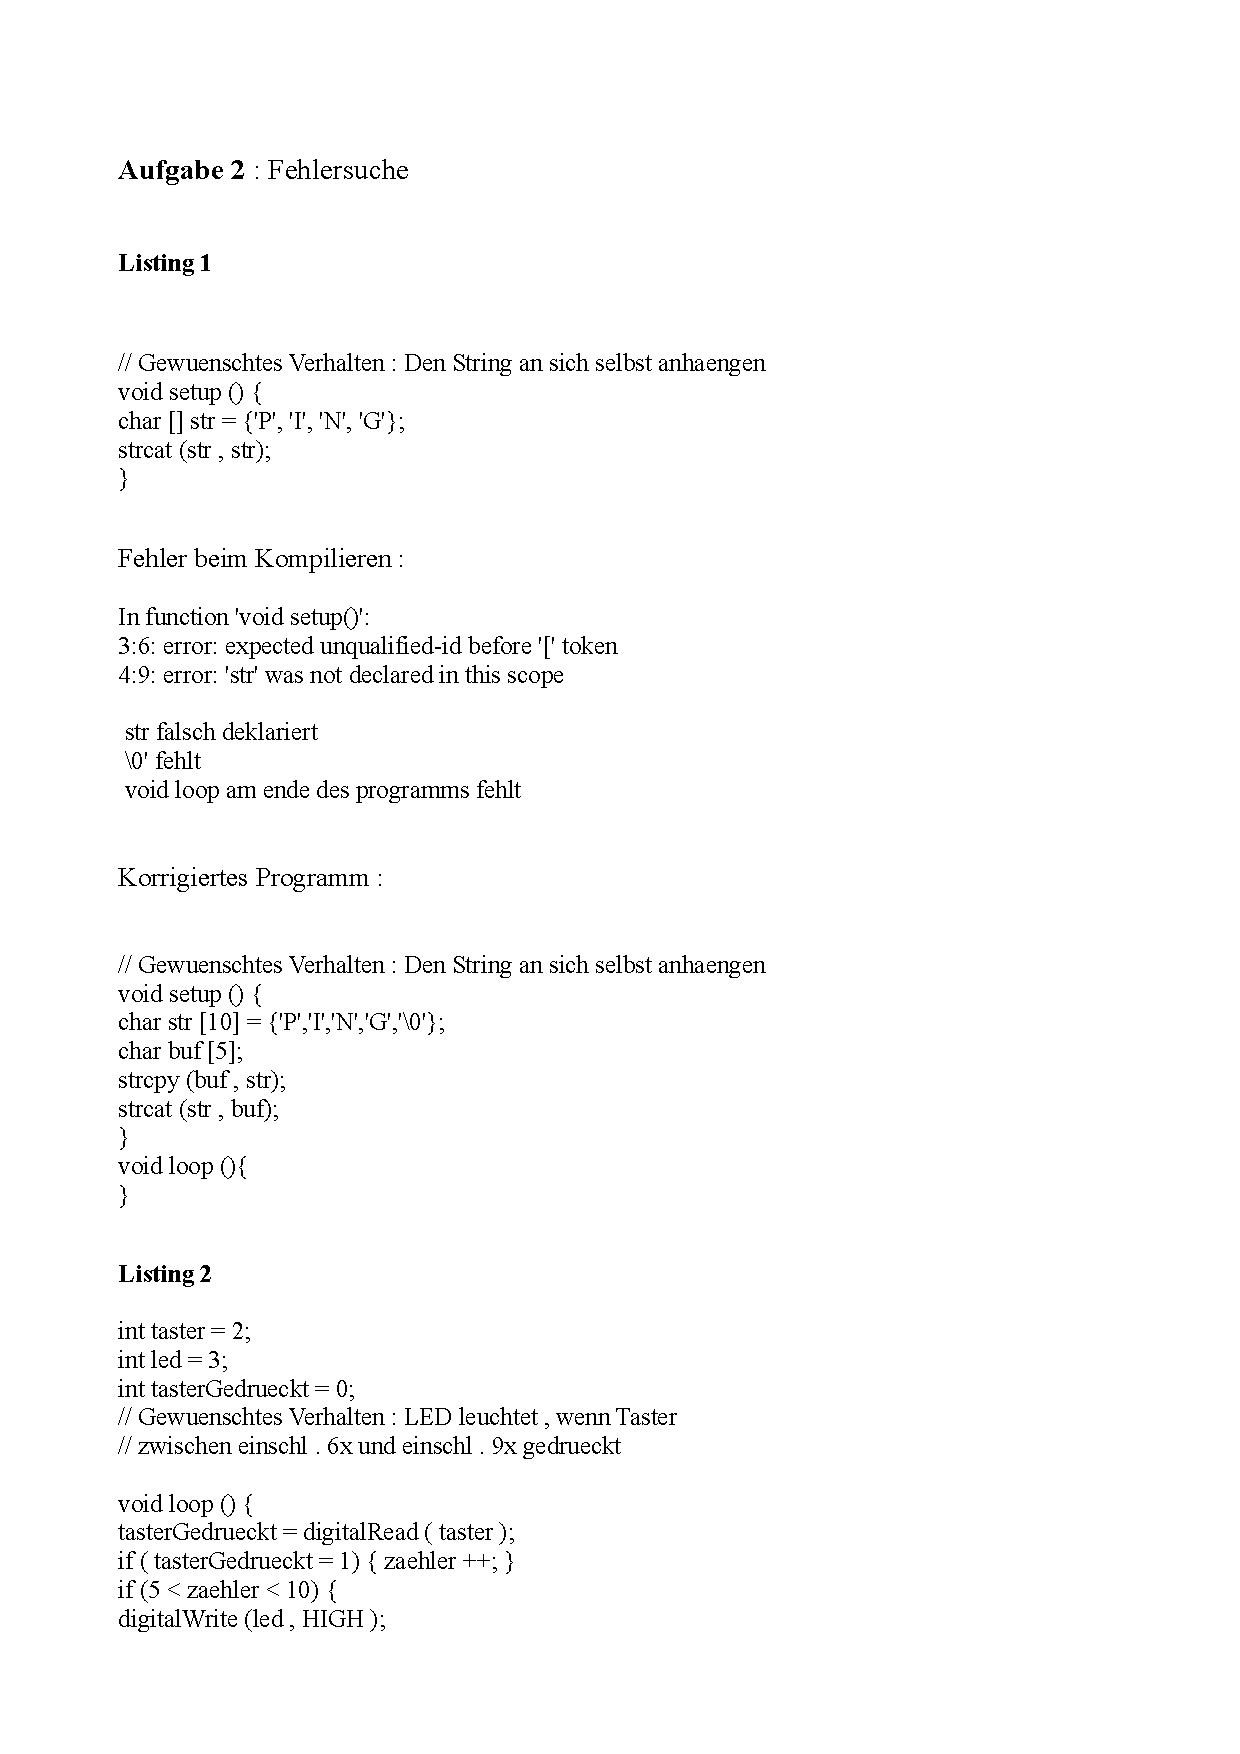
\includepdf[pages=-]{../Aufgabe2.pdf}

\end{document}
